\documentclass[BTech]{iitmdiss}
\usepackage{times}
\usepackage{epsf}
\usepackage{threeparttable}
\usepackage{float}
\usepackage{setspace}
\usepackage{amsmath}
\usepackage{amsthm}
\usepackage{txfonts,pxfonts,amsfonts}
\usepackage{epsfig}
\usepackage{caption}
\usepackage{subfig}
\usepackage{graphicx}
% \usepackage[square,numbers,sort]{natbib}
\usepackage[square]{natbib}
\usepackage[hypertex]{hyperref} % hyperlinks for references.
%\usepackage{algorithmic}
%\usepackage{algorithm}


%\include{commands}

% Strut macros for skipping spaces above and below text in tables. 
\def\abovestrut#1{\rule[0in]{0in}{#1}\ignorespaces}
\def\belowstrut#1{\rule[-#1]{0in}{#1}\ignorespaces}

\def\abovespace{\abovestrut{0.20in }}
\def\aroundspace{\abovestrut{0.20in}\belowstrut{0.10in}}
\def\belowspace{\belowstrut{0.10in}}
%%%%%%%%%%%%%%%%%%%%%%%%%


\def\thesistitle{Telemetry / Telecommand Frontend - IITMSAT}
\def\thesisauthor{Anoop R Santhosh}


\begin{document}
\bibliographystyle{iitm}
%%%%%%%%%%%%%%%%%%%%%%%%%%%%%%%%%%%%%%%%%%%%%%%%%%%%%%%%%%%%%%%%%%%%%% 
% Title page

\title{\thesistitle}

\author{\thesisauthor}

\date{May 2014}
\department{Computer Science and Engineering}

%\nocite{*}
\begin{singlespace}
\maketitle 
\end{singlespace} 



%%%%%%%%%%%%%%%%%%%%%%%%%%%%%%%%%%%%%%%%%%%%%%%%%%%%%%%%%%%%%%%%%%%%%%
% Certificate
\certificate

\vspace*{0.5in}

\noindent This is to certify that the thesis entitled {\bf {\thesistitle}}, 
submitted by {\bf {\thesisauthor}}, to the Indian Institute of Technology, 
Madras, for the award of the degree of {\bf Bachelor of Technology}, 
is a bona fide record of the research work carried out by him under my
supervision. The contents of this thesis, in full or in parts, have not been
submitted to any other Institute or University for the award of any degree or
diploma.

\vspace*{1.4in}
\hspace*{-0.25in}
\begin{singlespace}
\noindent {\bf Dr.~Shankar.~Balachandran } \\
\noindent Project Guide \\ 
\noindent Assistant Professor \\
\noindent Dept. of Computer Science and Engineering\\
\noindent IIT-Madras, 600 036 \\
\end{singlespace}
\vspace*{0.20in}
\noindent Place: Chennai\\ 
Date:

%%%%%%%%%%%%%%%%%%%%%%%%%%%%%%%%%%%%%%%%%%%%%%%%%%%%%%%%%%%%%%%%%%%%%%
% Acknowledgements
\acknowledgements

I would like to thank everyone who helped me.

%%%%%%%%%%%%%%%%%%%%%%%%%%%%%%%%%%%%%%%%%%%%%%%%%%%%%%%%%%%%%%%%%%%%%%
% Abstract

\abstract

\noindent KEYWORDS: \hspace*{0.5em} \parbox[t]{4.4in}{TMTC FrontEnd,
AX.25, IITMSAT}

\vspace*{24pt}

IITMSAT is a low orbit nano satellite being developed by students at IIT Madras. The satellite project has various subsystems both hardware and software . Ground Station software is an important part of it. TMTC front end is an important sub module within the ground station software. It essentially functions as the link layer and implements the link layer protocol which in this case is AX.25 .
\par The main functionality of this module include AX.25 protocol encoding/decoding , flow control including acknowledgements and counters and packet reassembly. The overall design is loosely inspired by the SwissCube ground station design. But to satisfy IITMSAT mission requirements which are different from SwissCube, many modifications are made, especially in the Telecommand transmitter part. The link layer protocol though based on standard AX.25 protocol, has been modified to meet our requirements. 


\pagebreak

%%%%%%%%%%%%%%%%%%%%%%%%%%%%%%%%%%%%%%%%%%%%%%%%%%%%%%%%%%%%%%%%%
% Table of contents etc.

\begin{singlespace}
\tableofcontents
\thispagestyle{empty}

\listoftables
\addcontentsline{toc}{chapter}{LIST OF TABLES}
\listoffigures
\addcontentsline{toc}{chapter}{LIST OF FIGURES}
\end{singlespace}


%%%%%%%%%%%%%%%%%%%%%%%%%%%%%%%%%%%%%%%%%%%%%%%%%%%%%%%%%%%%%%%%%%%%%%
% Abbreviations
\abbreviations
 
\noindent 
\begin{tabbing}
xxxxxxxxxxx \= xxxxxxxxxxxxxxxxxxxxxxxxxxxxxxxxxxxxxxxxxxxxxxxx \kill
\textbf{IITM}   \> Indian Institute of Technology, Madras \\
\textbf{RTFM} \> Read the Fine Manual \\
\end{tabbing}

\pagebreak

%%%%%%%%%%%%%%%%%%%%%%%%%%%%%%%%%%%%%%%%%%%%%%%%%%%%%%%%%%%%%%%%%%%%%%
%Notation

 \chapter*{\centerline{NOTATION}}
 \addcontentsline{toc}{chapter}{NOTATION}
 
 \begin{singlespace}
 \begin{tabbing}
 xxxxxxxxxxx \= xxxxxxxxxxxxxxxxxxxxxxxxxxxxxxxxxxxxxxxxxxxxxxxx \kill
 \textbf{$r$}  \> Radius, $m$ \\
 \textbf{$\alpha$}  \> Angle of thesis in degrees \\
 \textbf{$\beta$}   \> Flight path in degrees \\
 \end{tabbing}
 \end{singlespace}
 
 \pagebreak
 \clearpage

%The main text will follow from this point so set the page numbering
%to arabic from here on.
\pagenumbering{arabic}


%%%%%%%%%%%%%%%%%%%%%%%%%%%%%%%%%%%%%%%%%%%%%%%%%%
% Introduction.

 \chapter{INTRODUCTION}
 \label{chap:intro}
 
\par This chapter provides a brief introduction to IITMSAT in general and the particular problem statement i.e, TMTC Frontend .
 
 \section{Overview and Problem Statement}
 IITMSAT is a student initiated low orbit satellite project being developed at IIT Madras. A high energy particle detector is attached to the satellite and it can be used to measure changes in flux of charged particles in Ionosphere. The project aims to study the correlation between earth based phenomenon and the changes in charged particle flux. There are various subsystems involved in this project , both hardware and software . A detailed discussion of all the subsystems is beyond the scope of this document , though a few relevant parts will be briefly discussed here.   

\subsection {Overview of IITMSAT }
The main configurations/features of the satellite are as given below:
\begin{itemize}

\item \textbf{Orbit : } Low earth Orbit
\item \textbf{Altitude : } 600 km to 800 km
\item \textbf{Inclination : } \textgreater  45 degrees 
\item \textbf{Mission Life Time : } \textgreater 1 year 
\item \textbf{Dimensions : }  29 cm x 29 cm x 26 cm
\item \textbf{Mass : } 15 kg
\item \textbf{Payload : } High Energy Particle Detector 
\end{itemize}
 
 \subsection{Ground Station Software}
 Ground Station software is responsible for handling the operations of the satellite from ground and process the information transmitted by the satellite on downlink.It provides an interface for interacting with satellite and analysing data besides keeping track of various parameters of the satellite.The major modules with in the ground station software are : 
 
 \begin{itemize}
 \item \textbf{User Interface : }Lets the user select commands to control the satellite and displays various data collected by the satellite after processing and analysing it in appropriate ways.
 \item \textbf{Mission Control System }: MCS is responsible for converting the user inputs to CCSDS telecommands before dispatching them to the satellite . It is also responsible for archieving all packets send and received. It is also the unit which schedules commands and process the data received from satellite (CCSDS packets ) on downlink. It interacts which UIs on one end and TMTC frontend on the other. It transmits and receives CCSDS packets to/from TMTC Frontend.
 \item \textbf{TMTC Frontend : } This layer essentially performs like a link layer. It is discussed in detail below. 
 \end{itemize}
 
 \subsection{TMTC Frontend - The problem statement}
 TMTC Frontend essentially acts as a link layer between MCS and Satellite. The main aim of this project is to implement a robust TMTC Frontend. TMTC Frontend is responsible for encoding of CCSDS packets received from MCS and decoding of AX.25 frames received from GS. It is also responsible for handling Telecommand transmission  and Telemetry reception. It takes care of acknowledgments, packet resending etc. 
 
 
 \section{Motivation}
 
A robust link layer is very essential for proper communication with the satellite. This layer is responsible for encoding application data (CCSDS packets) to AX.25 protocol on uplink and vice versa on downlink.The communication link between earth based GS and satellite may not be very reliable. Hence we need a system which can take care of acknowledgements and resending of dropped packets without involving the application layer. This is important because the amount of time a communication link is open with the satellite in a day is very limited. So it is essential to handle packet resending ,acknowledgements and reassembly of received packets at this layer, rather than involving MCS (the application layer) which can slow down operations and affect the amount of data transferred. All data / command transfer between MCS and satellite happens through this layer.

\section{Contributions of this work}
Though the design is loosely based on GS Software design of Swisscube, there are quite a few differences. The transmission of data was not a big concern in case of Swisscube, which is not the case with IITMSAT. Hence in Swisscube GS software, resending dropped packets is handled at MCS through manual control. However, in case of IITMSAT, we expect to transmit more commands/ data in uplink and cannot depend on manual control for packet retransmission. So our design involves automated retransmission at link layer itself, instead of involving application layer. 
\par Another major difference from Swisscube is that we have modified the AX.25 frame to support 256 outstanding Telecommand packets at a time where as Swisscube design allows only for 4. Owing to the manual control over packet transmission , 4 outstanding packets was sufficient for Swisscube. But this is not the case with IITMSAT. 
 
 \section{Organisation of report}
 
This report is organised into 7 chapters. Chapter 2 explains a few terminology involved and frame structure of the protocols used. Chapter 3 gives a detailed explanation of the design of TMTC Frontend. Chapter 4 discusses  implementation details . Chapter 5 explains how the software system was tested. Chapter 6 is the Conclusion chapter . Chapter 7 is references. 

 \chapter{BACKGROUND AND PROTOCOLS}
 \label{chap:background}
This chapter gives a brief background on IITMSAT ground station software, detailed specifications of TMTC Front end and details of the protocol used.
\section{Ground Station Software}
As briefly mentioned in the introduction, ground station software is responsible for providing an interface to interact with the satellite and control the operations of the satellite from ground. The main user requirements are :
\begin{itemize}
\item Control the satellite and monitor its operations.
\item Process the downlink data and provide payload data in human interpretable format.
\item Monitor various house keeping parameters ,like voltage and alert user in case of issue or take actions whenever possible.
\item A GUI for easy human interaction.
\item Implement application layer protocols in compliance with ECSS standards. CCSDS packets are used for application data encoding. 
\item Provide a reliable communication channel to the satellite. 
\end{itemize}

Note : Within the CCSDS packet telemetry and telecommand concept
(CCSDS 102.0-B--5 to CCSDS 203.0--B--2), an on-board application process is defined as the source of telemetry source packets and the sink for telecommand packets.Through out this repot Telecommand refers to commands send to satellite from GS and Telemetry refers to data received by GS from satellite.

The GUI interacts with MCS. MCS can be considered the application layer. It is responsible for converting user commands into CCSDS packets , by reading commands and bit encoding from Mission Information Base(MIB) .Telecommands are defined in MIB.  MCS is also responsible for intelligent scheduling of Telecommands.It also archives all telecommands , telemetry and housekeeping data  in Mission Data Repository (MDR).
It is also responsible for decoding received telemetry(CCSDS packets) based on the encoding defined in MIB. It process the data  and displays it to the user in appropriate format through GUI.It can  be provided with support for processing payload data and represent it in human readable form or can just dump the payload data to some sink , which takes care of it.  It also keeps track of housekeeping parameters like voltage , on board time etc and alerts the user in case of an issue or take action when possible. It performs monitoring of the satellite completely. 

\par MCS interacts with users on one side, taking in commands and displaying received data. After processing the data and converting them to CCSDS packets, it forwards those packets to TMTC frontend. TMTC frontend as mentioned above forms a link layer and is responsible for encoding to AX.25 protocol and transmitting it to the satellite . This is the uplink part. On downlink , the MCS receives telemetery CCSDS packets from TMTC frontend. MCS then processes it , decodes data and takes appropriate actions or displays on GUI.

\section{TMTC Frontend}
TMTC Frontend is the layer between MCS and GS hardware. It acts as a link layer for communication between GS and satellite . It is expected to provide the following functionalities :
\begin{itemize}
\item \textbf{Uplink : } 
\begin{itemize}
\item Encoding CCSDS packets (Telecommand) to AX.25 frame.
\item Archive all telecommands.
\item Flow Control (resending, counters, acknowledgements etc ).

\end{itemize}
\item \textbf{Downlink : }
\begin{itemize}
\item Decode AX.25 frame (Telemetry) and reassemble the application data to obtain CCSDS packets.
\item Archive raw AX.25  telemetry frames. 

\end{itemize}
\item \textbf{Replay : }
\begin{itemize}
\item Provide functionality to replay archived raw AX.25 telemetry frames.
\end{itemize}
\end{itemize}
ADD IMAGE HERE USE CASE DIAGRAM
\linebreak TMTC frontend will be discussed in detail in next chapter.

\section{Data Link Layer Protocol -  \\ Modified AX.25 Frame structure }
AX.25 is a data link layer protocol derived from X.25 protocol suite and designed for use by amateur radio operators. AX.25 is most frequently used to establish direct point to point links.Since the overall IITMSAT design is based on Swiss cube design, we have decided to use AX.25 frames modified to meet our needs. Swiss cube uses their own modified version of AX.25. 

\par There are generally three types of AX.25 frames:
\begin{itemize}
\item  \textbf{Information Frame : }Used for data transfer.
\item \textbf{Supervisory Frame : }Used for supervisory link control.
\item \textbf{Unnumbered Frame : } Provides additional control over the link.
\end{itemize}
These frames can be distinguished by value of control field. The protocol and acknowledgement mechanisms which comes with this protocol does not suit our needs. For example , the protocol allows for only 8 outstanding packets, while our system needs more than 8 out standing packets.

\par We have decided to use only the frame structure of AX.25 protocol for our system and not the flow control mechanism described by the protocol. We have modified the frame structure to suit our needs by adding extra fields and changing the interpretation of some fields (from the standard protocol ).We are just using the frame encoding with our modifications and not any other feature. For the sake of convenience this modified version will still be referred to as AX.25 protocol/frame throughout this document. 
\par  The modified frame structure is briefly described below. The header common for both uplink and downlink will be discussed first, followed by modifications specific to each of them.

\subsection{Modified AX.25 Frame }
The frame structure is as shown below : 
\newline
\begin{figure}[H]

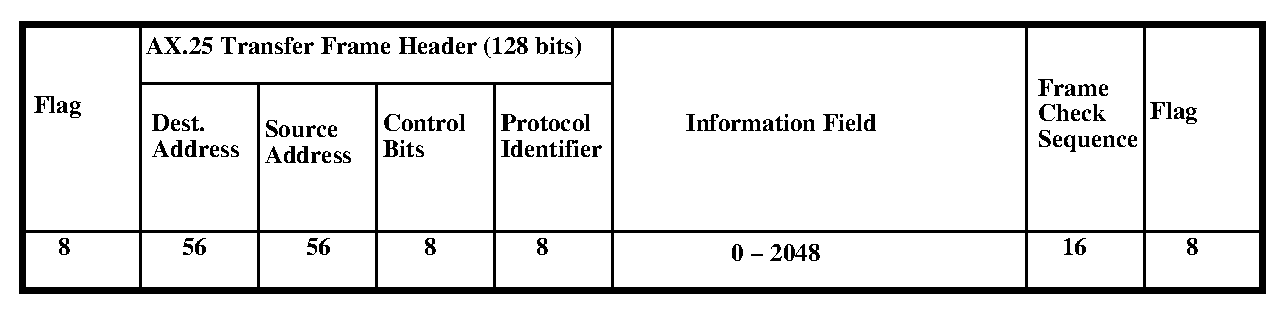
\includegraphics[scale = 0.65]{ax25main.eps.eps}
\caption{AX.25 Transfer Frame Format}
\label{fig:AX25mainframe}
\end{figure}
\\Few important  fields are briefly explained below :
\begin{itemize}
\item \textbf{Destination and Source Address : } Both have similar structure and length  56 bits. Destination and Source represents satellite or ground station depending on whether it is uplink or downlink. The address field structure is given below:
\newline
\begin{figure}[H]

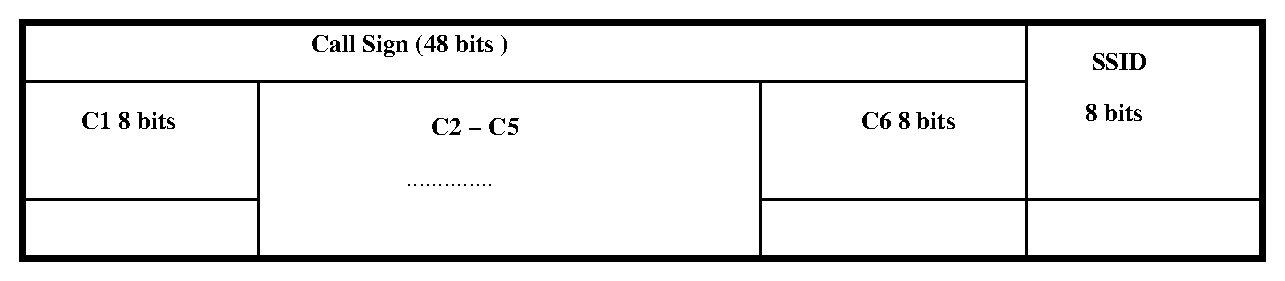
\includegraphics[scale = 0.65]{addressfield.eps}
\caption{AX.25 Address Field}
\label{fig:ax25addressfield}
\end{figure}

\\
\begin{itemize}

\item \textbf{CallSign : } 6 upper case letters.They are placed in C1 to C6 fields.
\item \textbf{SSID : } 4 bit integer used to identify multiple stations using the same call sign . They are placed in fields 3 to 6, with fixed values for other fields.
\end{itemize}
\item \textbf{Control bits : }8 bits long. Originally used to differentiate between the types of frames mentioned above, we no longer use it in our version. It is assigned a fixed value of 00000011 (0x03). This actually refers to an unnumbered frame. 
\item \textbf{Protocol Identifier : }8 bits long.Originally used to represent the layer 3 protocol used, we have modified this field to indicate if a frame is an acknowledgement frame. Value 00000011(0x03) indicates that it is an acknowledgement frame. Otherwise value is 11110000(0xF0) which as per standard protocol indicates no layer 3 protocol implemented.
\item \textbf{Frame Check Sequence : }CRC-CITT is used to calculate a 16 bit CRC. The polynomial used is x^{16}+x^{12}+x^{5}+1.


\end{itemize}

\subsection{Telecommand Information Field Usage }
To number the frames , the first byte of the information field is used as a  frame counter. Thus we have a modulo 256 counter for frames. Rest of the information field carries telecommand data , with a maximum size of 2040 bits or 255 bytes.Virtual channels are not supported on uplink.

\subsection{Telemetry Information Field Usage }
Telemetry information field has much more modifications than telecommand. An extra header and trailer are added. It supports virtual channels too. The information field structure is given below: 
\newline
\begin{figure}[H]
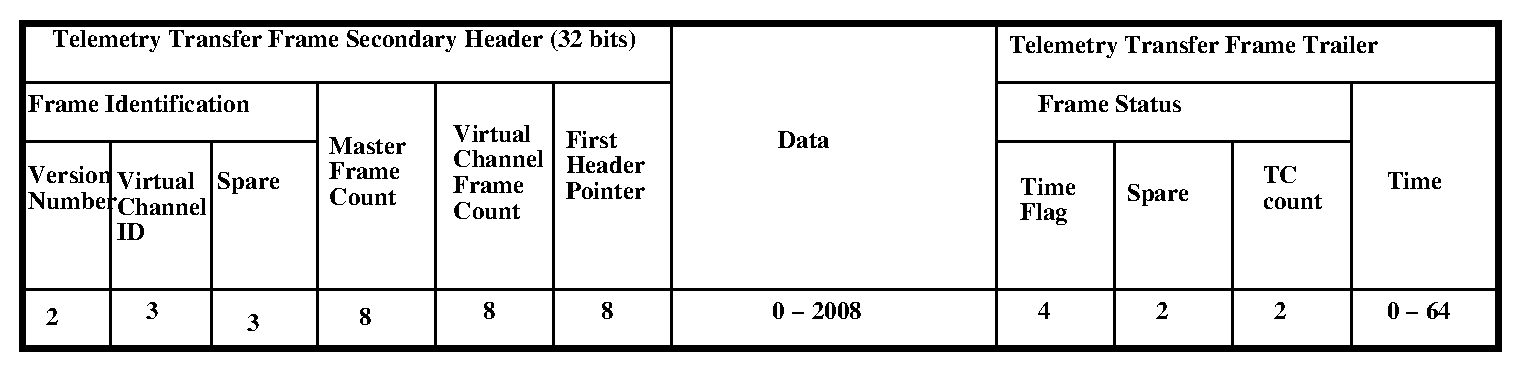
\includegraphics[scale = 0.5]{ax25telemetry.eps}
\caption{AX.25 Telemetry Header and Trailer }
\label{fig:ax25telemetry}
\end{figure}
\subsubsection{Secondary Header (32 bits) }
The secondary header is 32 bits long. It provides support for virtual channels and large data transfer (which will be discussed in detail later). The important fields are :
\begin{itemize}
\item \textbf{Frame Identification }
\begin{itemize}
\item Version Number (2 bits ) : Fixed to zero (00).
\item Virtual Channel ID (3 bits ) : Supports upto 8 virtual channels. Eg. 111 - represents data belongs to channel 8.
\item Spare (3 bits) : Reserved for future use. Value set to 000.
\end{itemize}
\item \textbf{Master Frame Count (8 bits)} : Total frame counter , ie., irrespective of the virtual channel. (modulo 256 counter).
\item \textbf{Virtual Channel Frame Count (8 bits ) }: Counter for a particular virtual channel (which corresponds to the current channel) . (modulo 256 counter ).
\item \textbf{First Header Pointer (8 bits) }: Specifies the octet number within data field that contains the first octet of the first packet header.Allows reassembly of packets even when previous packets were lost.
It has value 11111111(0xFF) if no packet header starts in the frame.


\end{itemize}

\subsubsection{Trailer (0 to 72 bits ) }
\begin{itemize}
\item \textbf{Frame Status (8 bits) }
\begin{itemize}
\item \textbf{Time flag (4 bits) : } Gives size of time field. 000 indicates no time field. If bit 0 is set to 1, bits 1 to 3 indicates the size of time field in octets + 1.
\item \textbf{Spare (2 bits ) :} Reserved for future application. Set to 00.
\item \textbf{TC Counter (2 bits ) :} No longer used in the modified version. Set to 00.

\end{itemize}
\item \textbf{Time (0 - 64 bits ) : }On Board time . Represents the time at which end flag of previous frame was transmitted.
\end{itemize}

\subsection{Acknowledgement Frame }
As mentioned earlier, a frame is identified as acknowledgement frame by value 0x03 in protocol identifier field. Individual packet numbers , each a byte long are placed sequentially in the informtaion field. An acknowledgement frame does not contain a counter (for telecommand )or telemetry header .

 \chapter{DESIGN OF TMTC FRONTEND}
 \label{chap:design}
 The TMTC Frontend consist roughly of four major sub modules.
\begin{itemize}
\item AX.25 Packet encoding/decoding
\item TC Transmitter
\item TM Receiver
\item Replay Controller
\end{itemize}
\section{AX.25 Packet encoding / decoding }
This module implements a library for encoding / decoding data to/from our modified AX.25 protocol frame structure. Frames are represented as a byte array. Implementation details will be discussed in next chapter.

\section{TC Transmitter}
The telecommand transmitter is based on a state machine.Initially it was decided to use to the Swiss cube transmitter algorithm. However it was quite limited for our requirements.
\subsection{Limitations of Swiss cube design}
\begin{itemize}
\item It can support only 4 outstanding packets.
\item Packets are transmitted one at a time.
\item Transmission is still manually controlled.
\item There was no option of resending at TMTC frontend layer.
\item In the event of packet drop, the information is carried back to the application level, where a human user decides to resend the packet again.
\item Even transmission of individual packets are triggered manually by user at MCS.

\end{itemize}

\subsection{Modified Design}
The manual control from application layer on transmission will make it really inefficient. No support for automatic resending of packets at TMTC layer also is an issue. This design was fine in case of Swiss cube , as they did not expect much data  transfer with the satellite. That is not the case  with IITMSAT. We expect to have more control over the satellite than Swiss cube and hence the above restrictions can be a serious concern.It slows down operations . This is especially important as IITMSAT plans to have only one ground station. This severely restricts the amount of time a communication link can be opened with the satellite as it comes into the field of view for a short time every day.Hence we modified the design to support more outstanding packets and support for resending at TMTC layer. The main characteristics are :
\begin{itemize}
\item Packets are sent when transmitter is on and positive beacon signal is received.
\item All the packets in the ready queue are dispatched at the same time one after another. The number of packets is expected to be in the order of 10, which is way less than the 256 outstanding packets allowed.
\item Transmitter is half duplex. So we are not implementing an expliict timeout. Acknowledgement for a frame send in a transmitter period is expected to come in the immediate next receiver period.
\item If acknowledgement is not received in the immediate next reception, packet is resend.A packet will be resend a fixed number of time, after which packet drop will be announced to MCS.

\end{itemize}

The state diagram is as given below :
\\ ADD IMAGE HERE \\
The states are :
\begin{itemize}
\item READY : Indicates that transmitter is ready to sent packets and transmitter is on. Positive beacon is the trigger to send frames.
\item WAIT\_FOR\_ACK : Waiting for acknowledgements of outstanding packets.If transmitter is turned on in this state, it adds all outstanding packets  to resend queue. If acknowledgement frame is received, state changes to WAIT\_FOR\_TRANS.
\item WAIT\_FOR\_TRANS :  Waiting for transmiter to switch on. When transmitter is on, moves to READY state.
\end{itemize}

The external triggers are :
\begin{itemize}
\item Transmitter ON : Indicates switch to transmission mode.
\item Transmitter OFF : Indicates switch to reception mode.
\item Positive Beacon : Indicates that satellite is in field of view and ready for reception.
\item Ack received : Indicates the reception of acknowledgement packet by receiver.

\end{itemize}

Besides this, the transmitter archives all AX.25 packets in a database with timestamp.
\section{Telemetry Receiver}
TM Receiver receives the telemetry from GS hardware (or in IITMSAT case , SDR ).Before going into details of how receiver process it , a few important concepts are discussed 
\subsection{Virtual Channels}
There are various subsystems on board the satellite which need to communicate with GS, like Housekeeping, payload  etc. All these subsystems require a communication link with GS, but only one physical data channel exists. The idea of virtual channels alleviate this problem. Each subsystem is assigned a virtual channel to communicate with ground station and these channels are multiplexed together into the same physical channel. Each frame has 3 bits to indicate which virtual channel the data  belongs to. Thus it can support up to 8 virtual channels . It gives an indication on how to process/forward  the data at GS . Also it gives all subsystems a fair chance of communication with GS. In the absence of virtual channels , a heavy subsystem like payload make occupy the master channel for most part, giving data light subsystems very less chance for communicating with ground station. Virtual channels ensure that all subsystems get a fair chance.Satellite just sends a packet with empty information field in case there is no data to be transmitted on that virtual channel in that particular slot.  As mentioned in previous chapter, the telemetry secondary header supports virtual channels. 
\begin{figure}[H]
\includegraphics[scale = 0.65]{vc.eps}
\caption{Virtual Channel}
\label{fig:vc}
\end{figure}
\subsection{Large Data Transfer and Reassembly Unit}
In case of telecommand ,it is quite possible to have commands of fixed size and it can usually be carried by the information field of a single AX.25 frame. This is not the case with Telemetry. Though we might be able to fix length of standard services, it is not possible in case of payload data. Payload data length can vary over a large range. Splitting payload data at application level is not good idea as it will lead to cumbersome processing later at MCS. This is the case with large payload packets. On the other side, payload packets could be quite small in size and more than one packet could fit into the information field of one AX25 frame. Transmitting them separately adds the header overhead to both the packets and it is  a waste of resources to do so. It would be better to fit in both of them into same AX.25 frame. Large Data Transfer Services help in solving these issues.The idea was proposed in [2].
\\ ADD CITATION \\
\par In large data transfer service, all the packets to be transmitted are sequentially attached one after another.This creates a single service data unit. This data unit is then split into fixed size (usually the size of information field of link layer protocol ) and each such unit are transmitted in each frame. 
\par Our design implements this service with the help of first header pointer in secondary header of AX.25 telemetry. This field indicates the octet in data field where the first byte of the header of first packet resides. Header of subsequent packets can be obtained after finding the length of each packet(We assume CCSDS packets and read the length from the predefined length field ). First header pointer helps in recovery of CCSDS packets even when the previous packets are lost. 
\par Reassembly unit is responsible for reassembly of packets at GS. There is a reassembly unit corresponding to each virtual channel. Reassembly unit takes care of packets arriving out of order. It maintains a buffer of all frames received on that channel and fills in data as and when the frames arrive , completing the packets. It creates a new buffer for each fragment of data and fills in the buffer when new frames arrive until the number of bytes specified by the length field is filled.

\subsection{Overall design of TM Reeciver}
Processing steps after reception of an AX.25 Telemetry frame in that order is as follows. 
\begin{enumerate}
\item Receive AX.25 frame.
\item CRC check to detect frame bit errors.
\item Check the GS and Satellite SSID and Callsign.
\item If the frame is an acknowledgement frame, trigger Acknowledgement received of receiver.
\item Otherwise Archive the raw frame in database .
\item Forward the frame to appropriate virtual channel.
\item Transfer the frame to reassembly unit of the virtual channel.
\item After a CCSDS packet is completely reassembled, forward it to the MCS on appropriate port or channel. 
\end{enumerate}

\section{Replay Controller}
Replay controller lets the user replay archived AX.25 raw frames. It provides a small GUI where user can enter the virtual channel ID and the time range of in which the packets he/she wants to replay was received by the receiver. Replay controller reads all frames in the range for that particular virtual channel from the database. It then creates a reassembly unit and forwards the frames one by one to the unit. Upon completion packets are forwarded to MCS as usual.
%%%%%%%%%%%%%%%%%%%%%%%%%%%%%%%%%%%%%%%%%%%%%%%%%%%%%%%%%%%%
% Appendices.

 \appendix
 
 \chapter{A SAMPLE APPENDIX}
 
 Just put in text as you would into any chapter with sections and
 whatnot.  Thats the end of it.

%%%%%%%%%%%%%%%%%%%%%%%%%%%%%%%%%%%%%%%%%%%%%%%%%%%%%%%%%%%%
% List of papers

\chapter*{Publications}
\vspace{-0.3cm}

\begin{enumerate}
\item S. M. Narayanamurthy and B. Ravindran (2007). \newblock
  Efficiently Exploiting Symmetries in Real Time Dynamic Programming. \newblock {\em
  IJCAI 2007, Proceedings of the 20th International Joint Conference on
  Artificial Intelligence}, pages 2556--2561.
\end{enumerate}

%\nocite{bellman, Amarel:1968, manning, knoblock90learning,
%crawford92theoretical, Barto:rtdp, Ravindran:proof}

%%%%%%%%%%%%%%%%%%%%%%%%%%%%%%%%%%%%%%%%%%%%%%%%%%%%%%%%%%%%
% Bibliography.
\pagebreak
\begin{singlespace}
  \begin{small}
	\bibliography{refs}
  \end{small}
\end{singlespace}

%%%%%%%%%%%%%%%%%%%%%%%%%%%%%%%%%%%%%%%%%%%%%%%%%%%%%%%%%%%%

\end{document}
